\section{Visual Perception}

\textbf{Gestalt principles}


Gestalt psychology was founded in the 1920s by Max Wertheimer and others. It is about the perception of groups, patterns and objects. \medskip

\textit{Four key principles}
\begin{multicols}{2}
    \begin{itemize}[itemsep=-5pt, topsep=0pt, leftmargin=*]
        \item Emergence
        \item Multistability
        \item Reification
        \item Invariance
    \end{itemize}
\end{multicols}

\textit{Laws of grouping}
\begin{itemize}[itemsep=-5pt, topsep=0pt, leftmargin=*]
    \item Proximity (close objects belong to group)
    \item Similarity (similar appeareance belong to group)
    \item Closure (humans prefer to see complete figures)
    \item Symmetry (Symmetric objects form groups around the center)
    \item Figure and ground (users tend to seperate images to fore- and background)
    \item Continuity (Objects that intersect are perceived as continous rather than individual objects)
    \item Past experience (Based on past experience group objects together)
\end{itemize}
\medskip

\textbf{Feature integration theory} \smallskip

Availability of visual information is limited. Full visual acuity is only available in foveal area. Peripheral vision provides limited information. 
This is why FIT suggests stimuli that are registered early and automatically. 

\begin{center}
	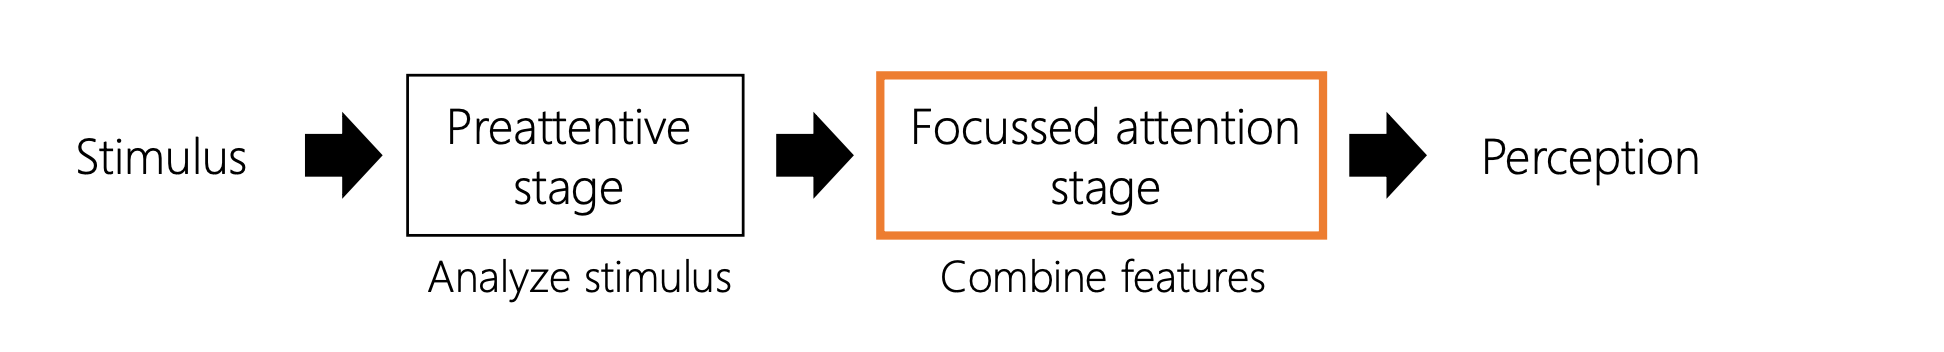
\includegraphics[width=\linewidth]{feature_integration_principle.png}
\end{center}
\begin{center}
	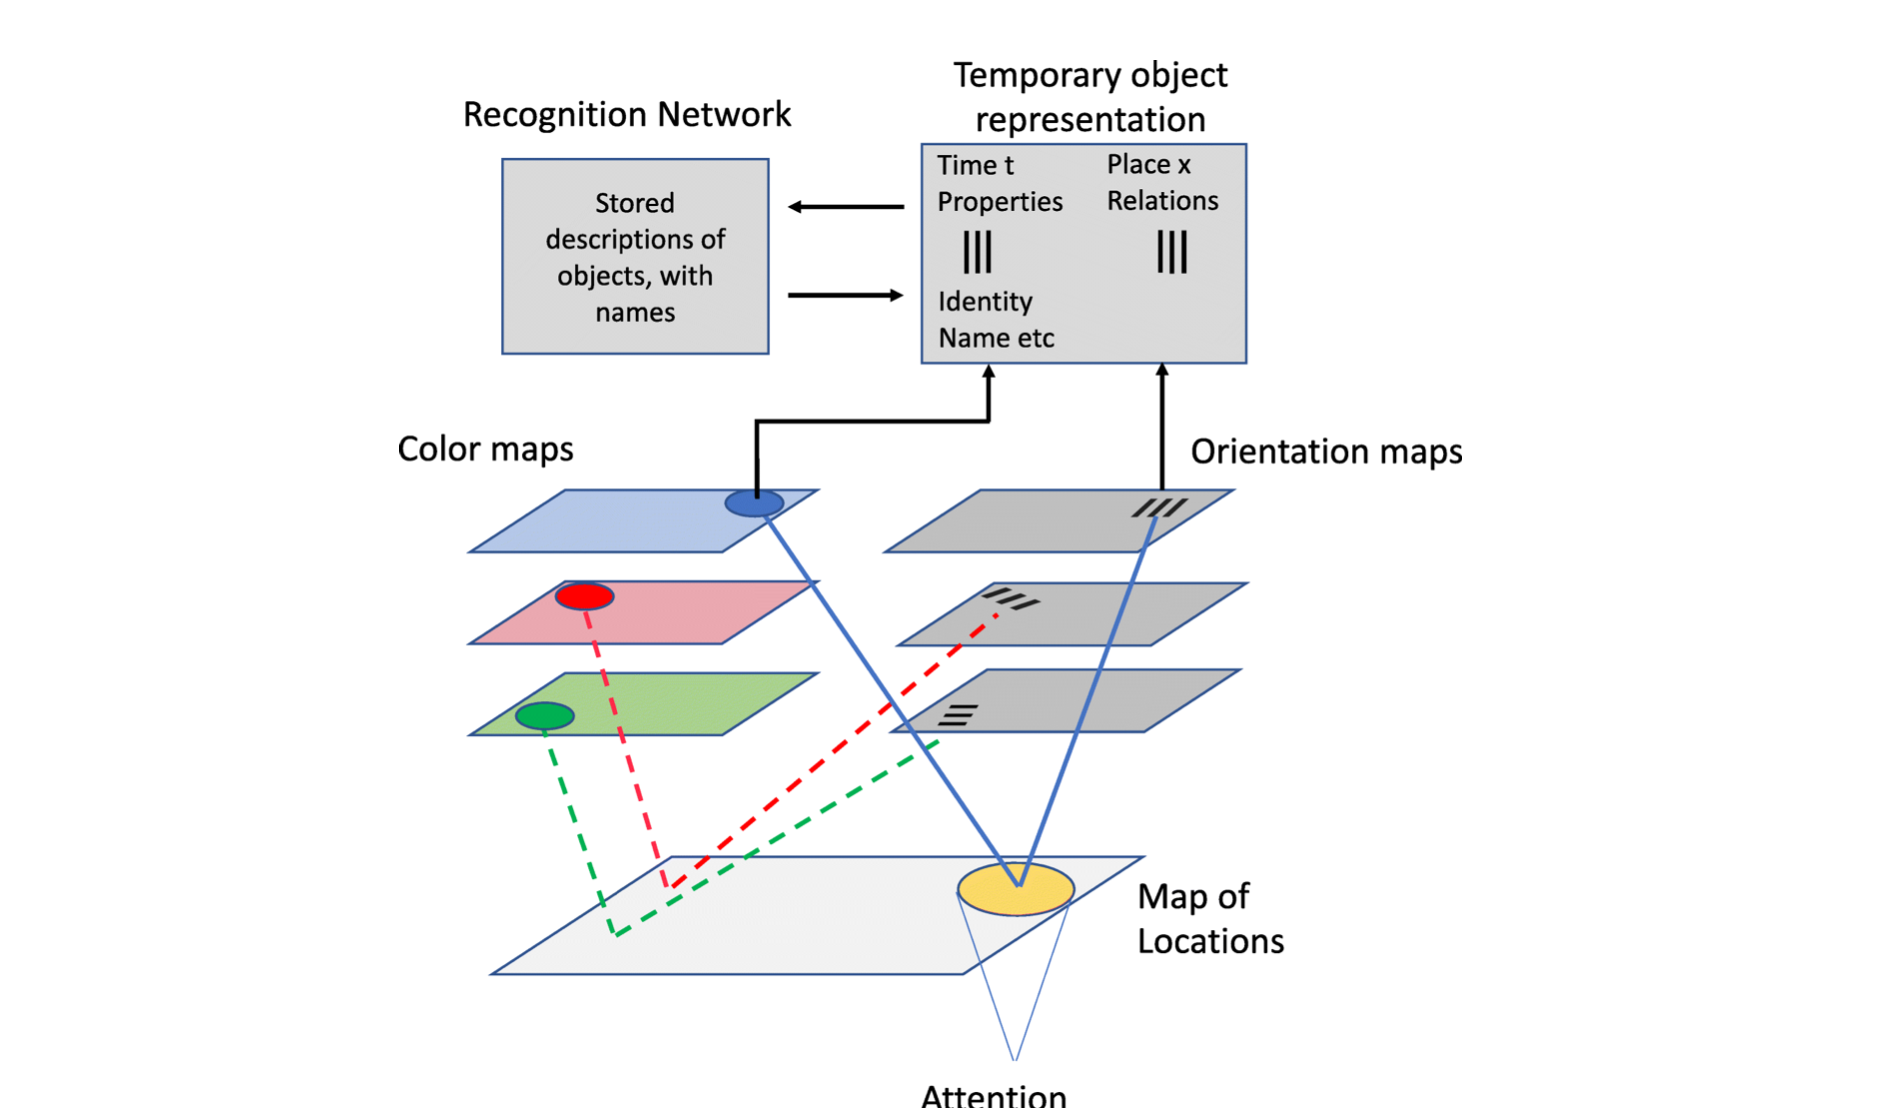
\includegraphics[width=\linewidth]{fit_2.png}
\end{center}

Theory is based on the process of selective attention. Is useful but certainly limited in certain aspects. FIT primarily concerns bottom-up activation. Top-down activation through memory and expectation. \medskip

\textbf{Selective Attention} \smallskip

There is an ongoing debate about Early / Late selection. The early selection model has been proposed earlier and mainly relies on the idea of an early "bottleneck" in the attentional process given by perception. 
It also assumes that focussed attention can prevent distractor processing at an early stage\medskip

Late selection was proposed later and assumes unlimited perception and the automatic discrimination of relevant and irrelecant stimuli. 
It assumes that later processes such as memory or behavior are the processes with selected attention. \medskip

\textbf{Perceptual Load Theory} \smallskip

Sees perception as a process with limited capacity. This is in line with the early selection views. PLT also assumes that all stimuli are automatically processed until capacity is filled. \smallskip

\textit{Example experiment on PLT}
\begin{center}
	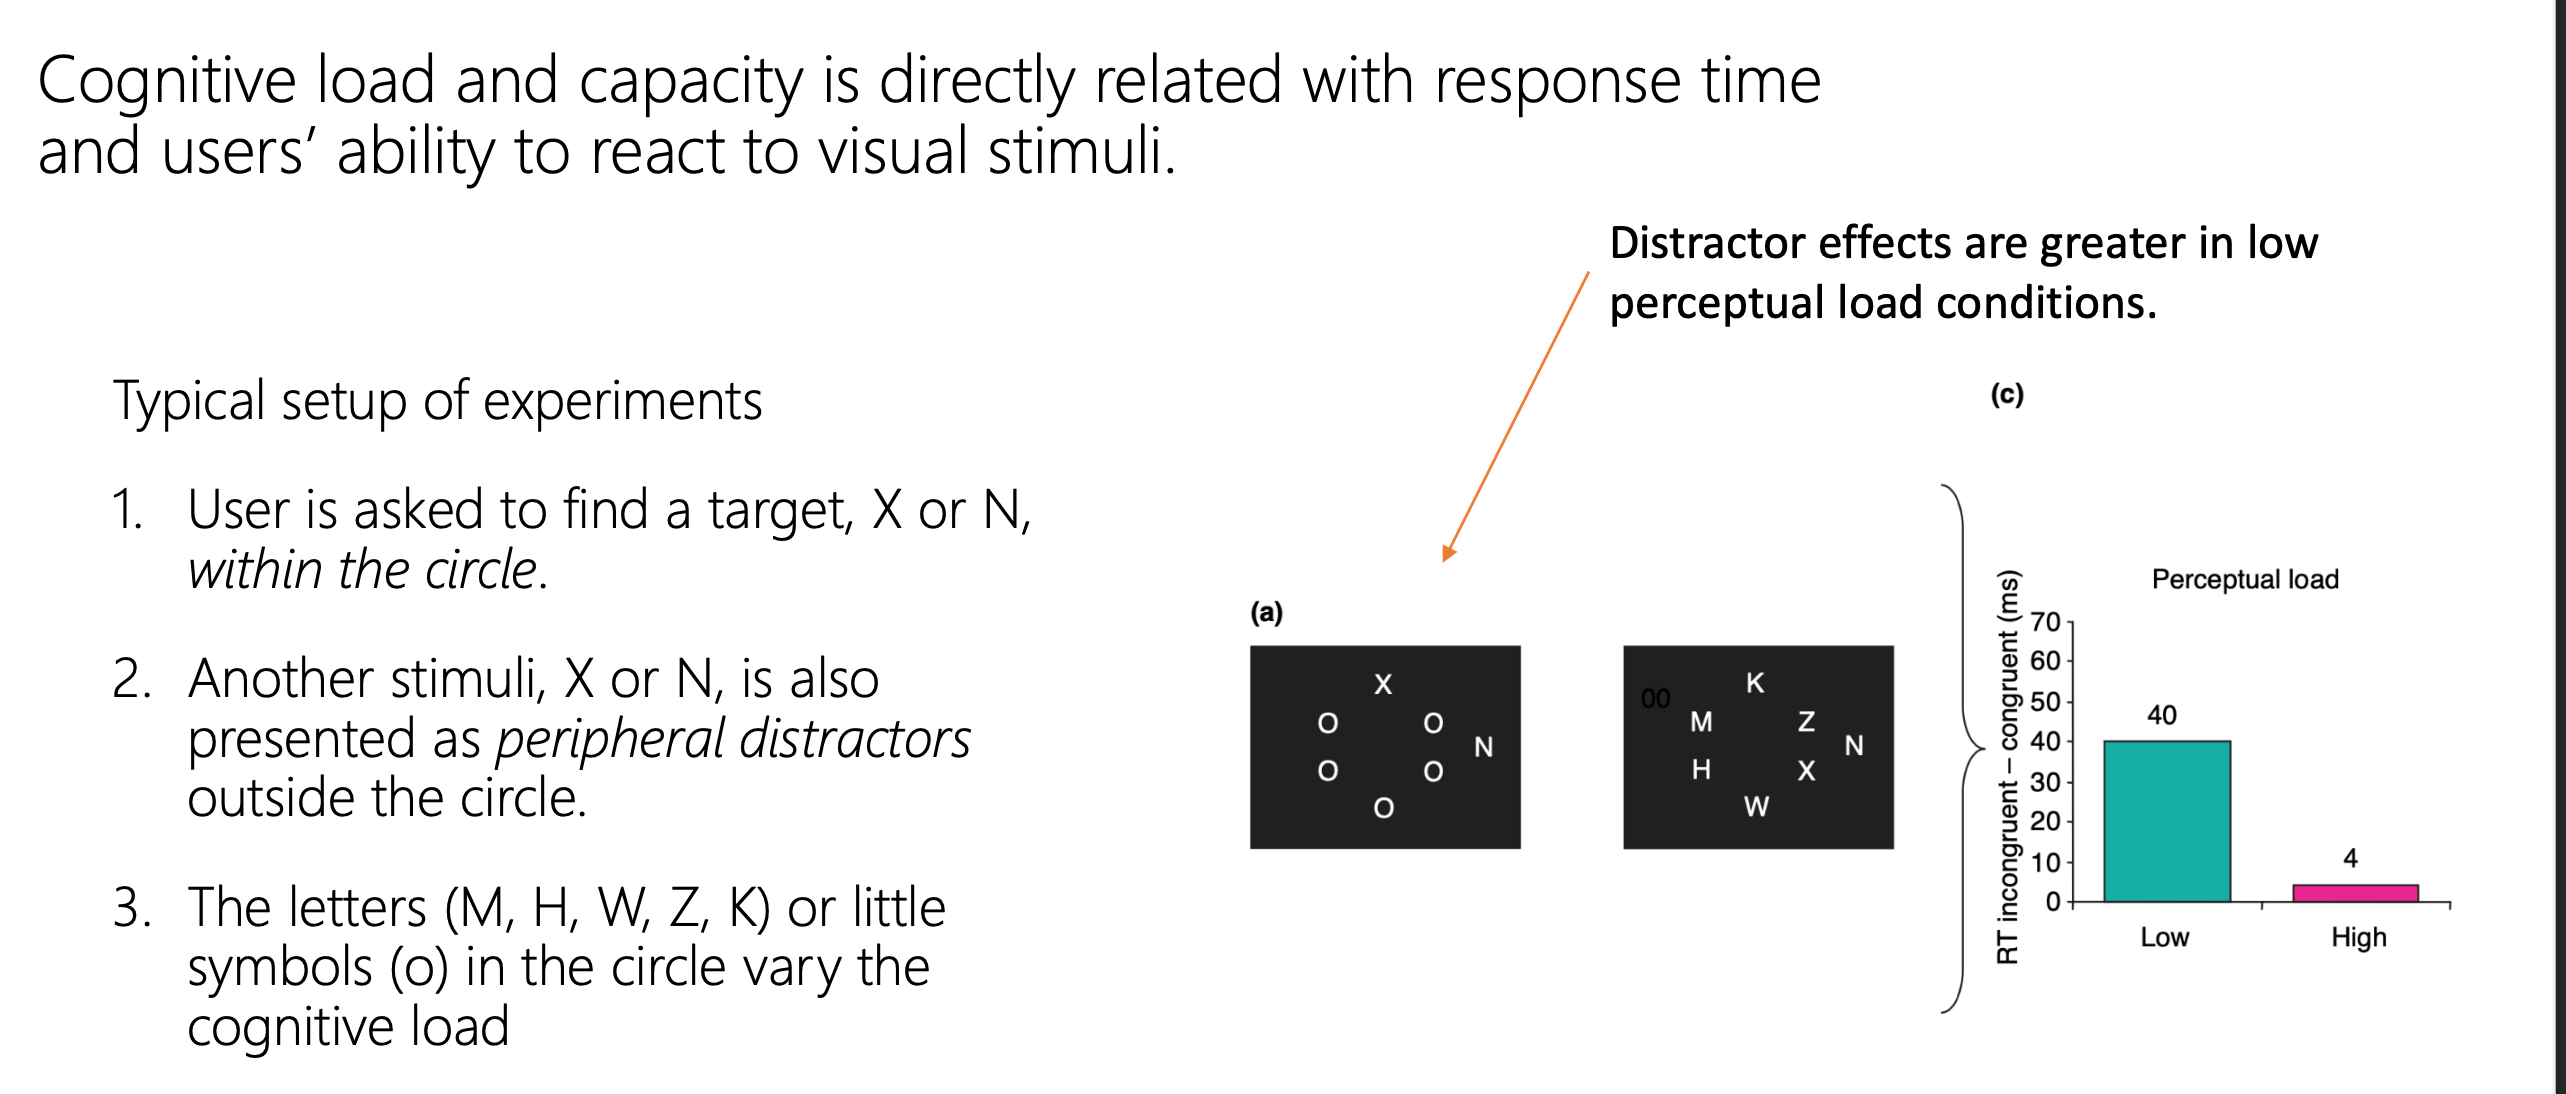
\includegraphics[width=\linewidth]{plt_experiment.png}
\end{center}

\textit{Takeaways on PLT}

Users ability to react to stimuli is related to its context. High load leads to more focus and less distraction. Low load leads to quicker distraction.\medskip

\begin{center}
	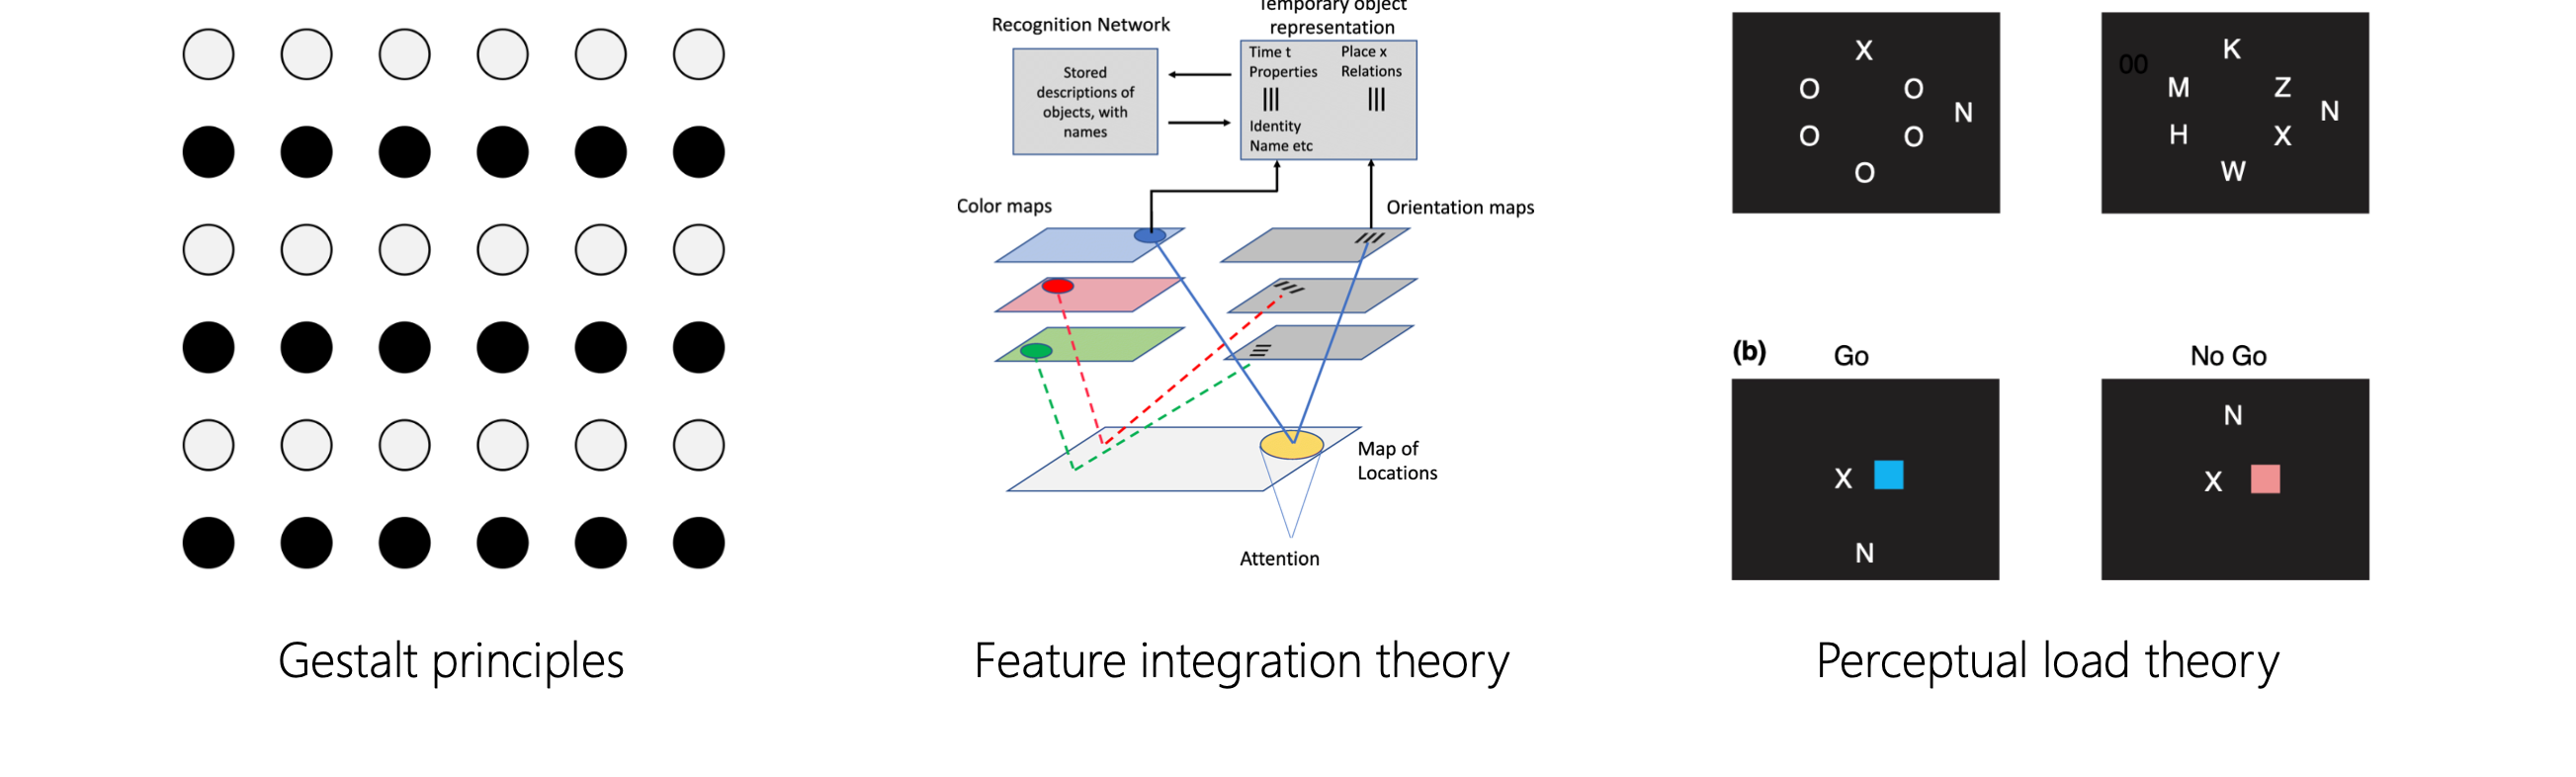
\includegraphics[width=\linewidth]{models_of_perception.png}
\end{center}

\textbf{Visual Saliency} \smallskip

The context of objects popping-out as pre-attentive for selection. Assumes that feature maps are computed in parallel and combined. The computed maps yield a saliency map. Assumes that the "Winner-takes-it-all".
Assumes that this sequential processing is based on inihibition of return. \medskip

Example is given by an experiment where different skins are compared and snake skin resulted in significantly higher brain activity measured over EEG. \smallskip

With visual saliency we can predict users' gate and importance. It is mainly bottom-up and therefore feature based. Top-down saliency is challenging, however task and load influence the saliency. \medskip

If there is too many competing features, clutter will occur. \medskip


\begin{center}
	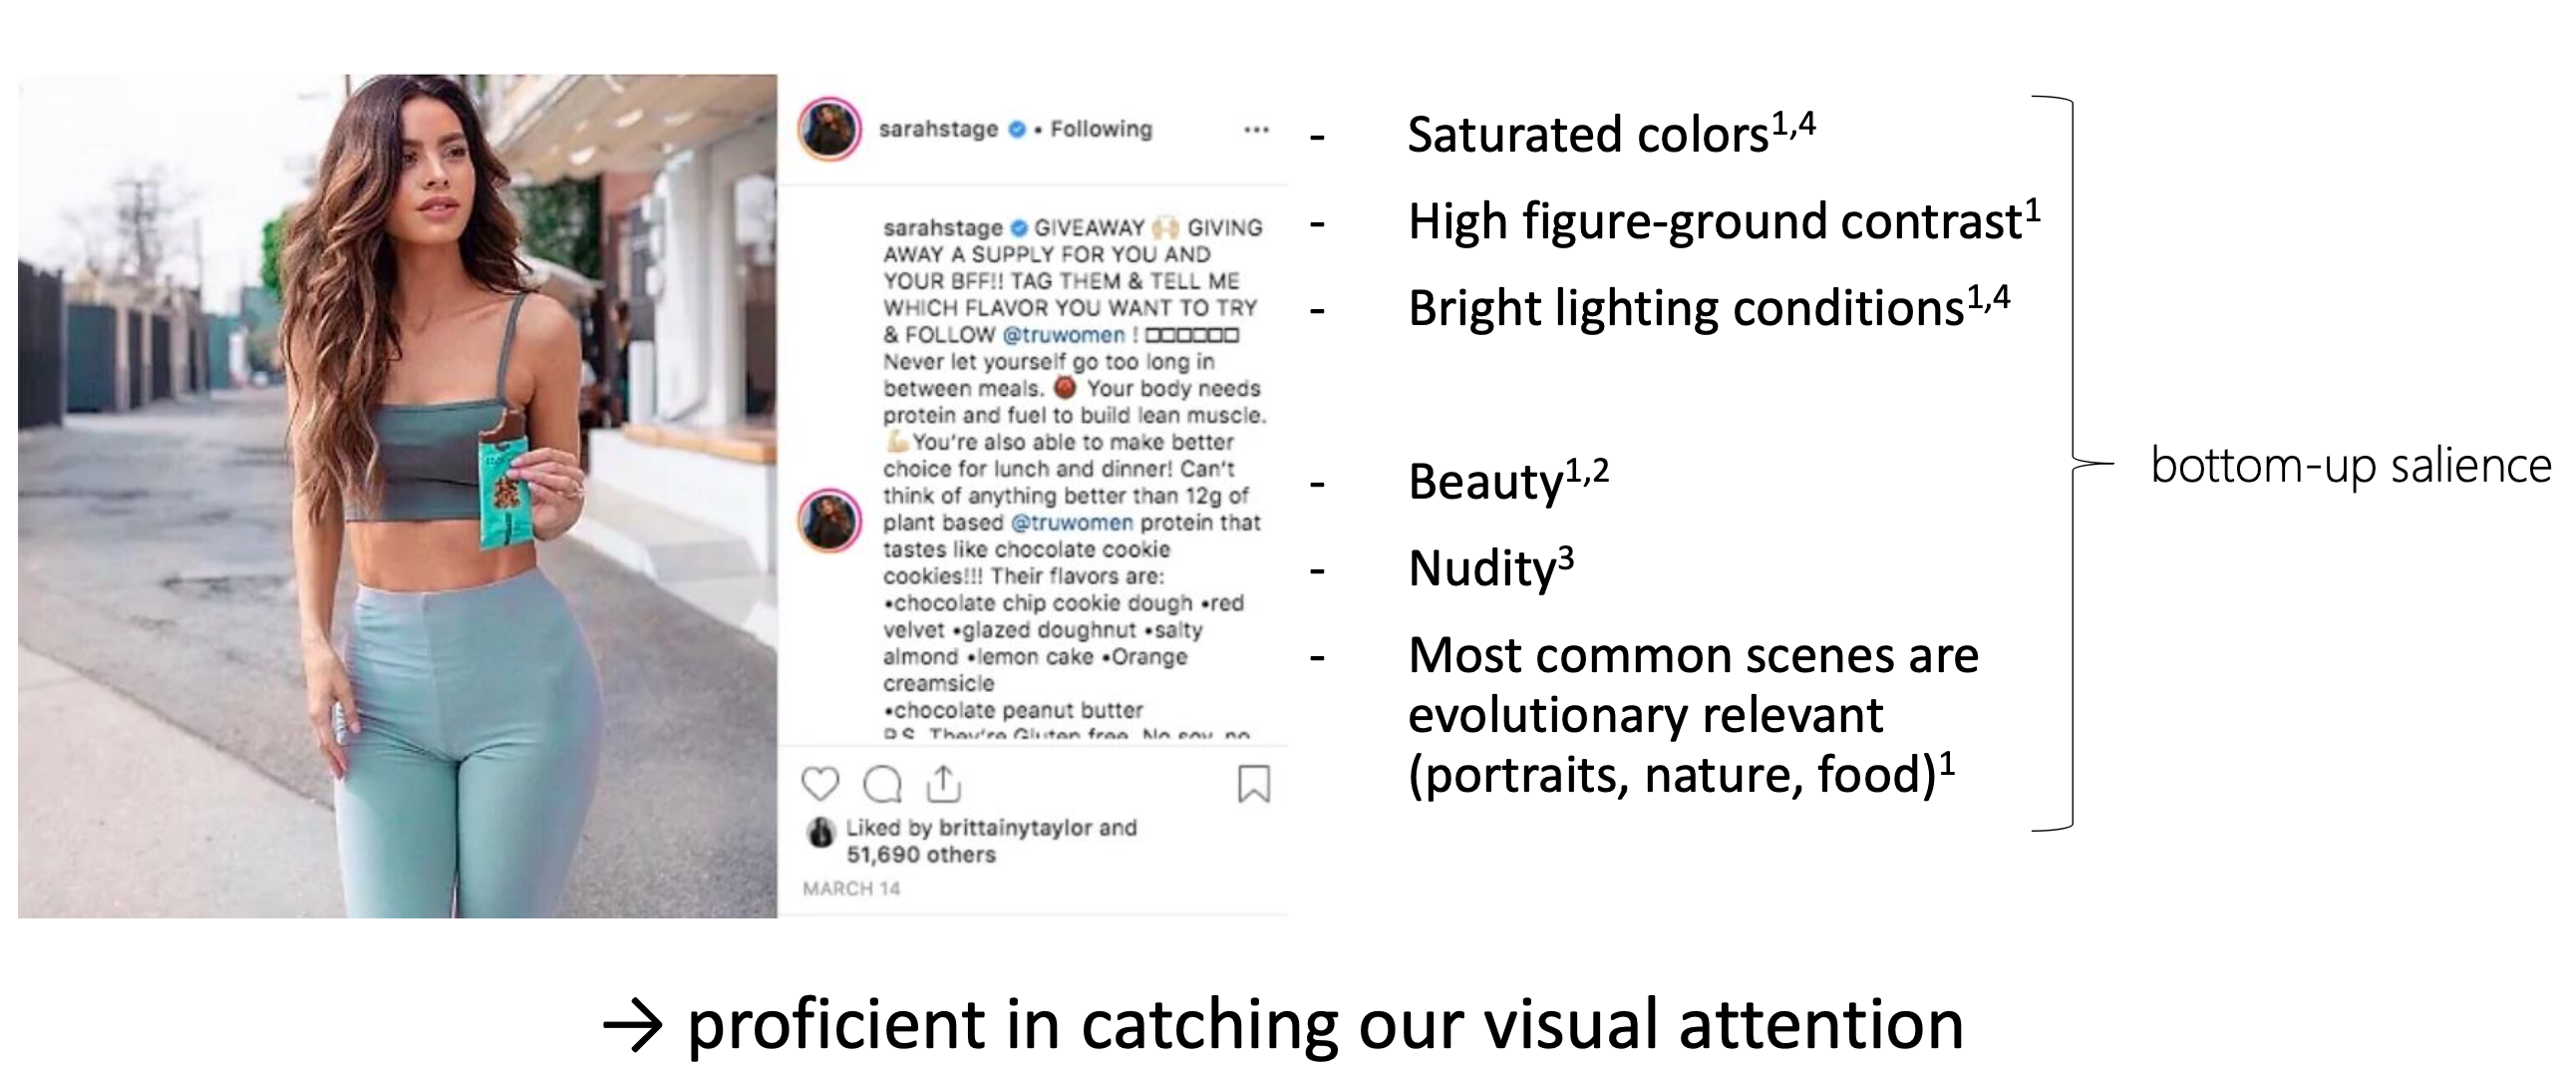
\includegraphics[width=\linewidth]{visual_saliency_example.png}
\end{center}



\textbf{Visual Search} \smallskip

The process that decides where humans look next. 

\begin{enumerate}[itemsep=-5pt, topsep=0pt, leftmargin=*]
    \item Guided Search (rules exist on priorities for items or areas int the scene)
    \item Bounded rationality (selection of actions based on expected utility bunder uncertainty)
\end{enumerate}

\medskip

\textit{Guided Search} \smallskip

\begin{enumerate} [itemsep=-5pt, topsep=0pt, leftmargin=*]
    \item Calculate the distance (eccentricity) to the current fixation location for each item
    \item Given eccentricity, decide which items and features are available to visual representations
    \item Calculate bottom-up saliency for each item
    \item Calculate top-down saliency for each item
    \item Sum up bottom-up and top-down activations and select the ones with highest activation
\end{enumerate}

\textit{Bounded Rationality} \smallskip

Assumes that humans take the action with satisfactory expected utility given their constraints. 

\begin{center}
	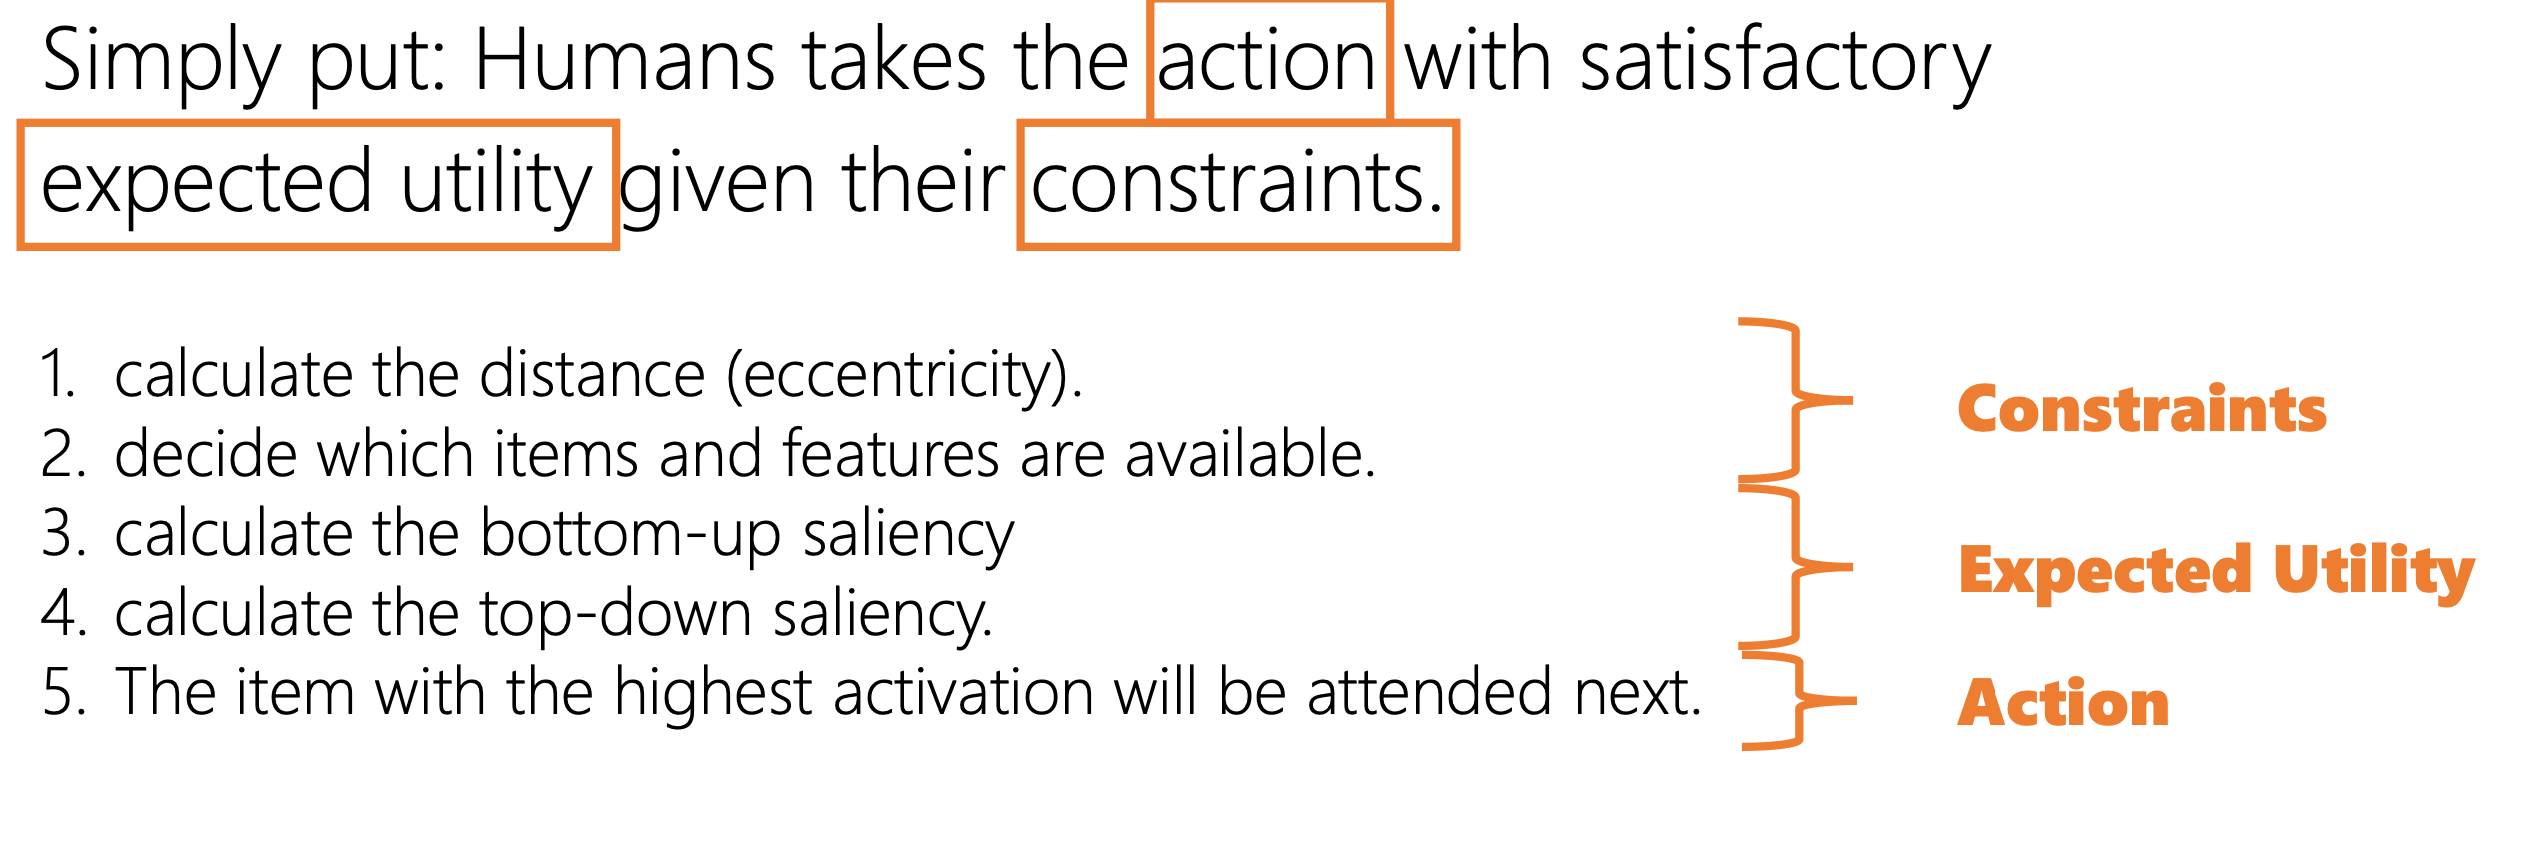
\includegraphics[width=\linewidth]{bounded_rationality.png}
\end{center}

Both visual saliency and search behavior are important for user interfaces and computational design. \medskip

\textbf{Application in HCI} \smallskip

\textit{Aalto interface metrix (AIM)} \smallskip

Combination of empirical models and metrics of user perception and attention. 
Quantifies user experience, complements and removes guesswork. \medskip


\textit{Online UI adaption} \smallskip

Is a tool to measure spatially and semantically relevant labels. Measures pre-attentive object features. It is also possible to distinguish pre-attentive and attentive object features. \medskip

There are also many more tools and applications that make use of these concepts. 

\columnbreak


